\chapter{Umsetzung} \label{sec:Umsetzung}
Im folgenden Kapitel wird die Umsetzung beschrieben.

\section{Datenbankschema}\label{db:DB}\chapterauthor{Dominic Steinhauser}
Innerhalb der SQLite Datenbank werden die Tabellen DHT, MQ135, Security und Window angelegt. Dadurch können die Sensordaten strukturiert in Tabellen gespeichert und die Werte mithilfe von \acf{SQL} leicht abgefragt werden. Die vier Tabellen sind auf die Anforderungen F-10.1, F-10.2, F-10.3 und F-10.4 zurückzuführen, sodass jeder Sensor seine Werte in eine eigens dafür angelegte Datenbank schreibt. Der Vorteil davon ist, dass die Übersichtlichkeit der von einem Sensor erzeugten Daten gewährleistet ist.\\
Jede Tabelle besitzt pro Relation eine eindeutige ID. Dies hilft einen Datensatz eindeutig zu identifizieren. Neben der ID kann der Timestamp ebenfalls als eindeutige Identifizierung eines Datensatzes genutzt werden, da es sehr unwahrscheinlich ist, dass innerhalb einer Millisekunde zwei Datenbankeinträge in einer Tabelle erstellt werden.\\

Daten aus dem DHT22 Sensor (Temperatur- \& Luftfeuchte) werden in der Tabelle DHT in den folgenden Spalten abgespeichert:
\begin{itemize}
	\item \textbf{ID}: Primärschlüssel, der nicht leer sein darf und sich inkrementell erhöht.  
	\item \textbf{Temperature}: Temperaturwert in Celsius wird als REAL Number gespeichert.
	\item \textbf{Humidity}: Prozentwert der Luftfeutchtigkeit wird als REAL Number gespeichert.
	\item \textbf{Sensorid}: Text, der angibt um welche Art von Temperatur- \& Luftfeuchtigkeitssensor es sich handelt.
	\item \textbf{Timestamp}: Zeitstempel wird in Millisekunden als Integer gespeichert
\end{itemize}

Die Window Tabelle nimmt die Werte des Magnetkontakts entgegen und speichert diese:
\begin{itemize}
	\item \textbf{ID}: Primärschlüssel, der nicht leer sein darf und sich inkrementell erhöht.  
	\item \textbf{Value}: Integer, entweder 1 für geöffnetes Fenster oder 0 für geschlossen.
	\item \textbf{Timestamp}: Zeitstempel wird in Millisekunden als Integer gespeichert
	\item \textbf{Room}: Beschreibung, in welchem Raum der Fensterstatus geprüft wird. 
\end{itemize}

Der MQ-135 Sensor speichert die verschiedenen Werte der Gase CO2, CO und NH4 in folgenden Spalten ab.
\begin{itemize}
	\item \textbf{ID}: Primärschlüssel, der nicht leer sein darf und sich inkrementell erhöht.  
	\item \textbf{CO2}: CO2 Wert in parts per million (ppm) wird als REAL abgespeichert.
	\item \textbf{CO}: CO Wert (ppm) wird als REAL abgespeichert.
	\item \textbf{NH4}: NH4 Wert (ppm) wird als REAL abgespeichert. 
	\item \textbf{Timestamp}: Zeitstempel wird in Millisekunden als Integer gespeichert
\end{itemize}

Sobald die Bibliothek Motion eine Bewegung erkennt, wird automatisch ein Datenbankeintrag generiert der die nachfolgende Struktur aufweist:
\begin{itemize}
	\item \textbf{ID}: Primärschlüssel, der nicht leer sein darf und sich inkrementell erhöht.  
	\item \textbf{Camera}: Integer, der angibt welche Kamera das Bild aufgenommen hat.
	\item \textbf{Filename}: Text, der angibt unter welchem Pfad das Bild gefunden werden kann.
	\item \textbf{Frame}: Integer, der angibt welches aus dem Video extrahiert wurde. 
	\item \textbf{File\_type}: Integer, der angibt um was für eine Datei es sich handelt.
	\item \textbf{Timestamp}: Zeitstempel, der als im Format \enquote{YYYY-MM-DD HH:MM:SS} angibt, wann die erste Bewegung erkannt wurde.	
\end{itemize}


\section{Raspberry Pi} \chapterauthor{Dominic Steinhauser}
Im folgenden Abschnitt wird beschrieben, wie der Raspberry Pi mit den Sensoren interagiert, die Daten speichert und anschließend über Services bereitstellt.

\subsection{Sensor Adapter - Datenbeschaffung}
Der Raspberry Pi bildet die zentrale Einheit, um verschiedene Sensoren in eine Anwendung zu integrieren. Dabei spielen dessen externe Schnittstellen eine wesentliche Rolle. Allerdings liegt der Fokus dieser Arbeit auf der Datenbereitstellung über einen Webserver, dem Verarbeiten und Anzeigen in der App, weshalb teilweise auf bereits bestehende Lösungen zurückgegriffen wird.
\\\\Das \acf{CSI} stellt eine Möglichkeit dar, eine eigens für den Raspberry Pi entworfene Kamera anzuschließen. Das Kameramodul kann dann über entsprechende Befehle über die Kommandozeile des Raspberry Pis gesteuert werden. Aus der Anforderung F-10.1 geht hervor, dass Bilder bei erkannter Bewegung gespeichert und einen Livestream umgesetzt werden sollen.\\Die Anzeige eines Live-Bildes könnte über eine sekündliche Aufnahme, die über eine Service unter einer Internetadresse verfügbar gemacht wird, umgesetzt werden. Ob innerhalb eines Bildes Bewegung erkannt wird, könnte durch eine Vergleich eines Referenzbildes und dem aktuellen Bild ermittelt werden.\\Allerdings bietet diese Funktionalitäten bereits das Open-Source Programm \enquote{Motion} an. Es ist in der Lage Bewegung zu erkennen, Live-Bilder anzuzeigen und erkannte Bewegung in Form von Events abzuspeichern.\cite{motion:Motion}\\
\\Motion wurde so konfiguriert, dass der Livestream über die \ac{IP}-Adresse des Raspberry Pis und dem Port 8081 erreichbar ist. Eine Bewegung wird erkannt, wenn sich drei aufeinanderfolgenden Bilder um 15000 Pixel zum Referenzbild unterscheiden. Dabei ist eine Auflösung von 640x480 Pixel gewählt. Wenn für sieben Sekunden keine Bewegung mehr wahrgenommen wird, ist das Event beendet. Für jedes Event wird in der Tabelle Security (siehe \autoref{db:DB}) ein Datenbankeintrag erstellt. Außerdem wird ein Video in einem definierten Verzeichnis abgespeichert, das die ganze Sequenz der Bewegungserkennung enthält. Nachdem das Video erstellt wurde, wird außerdem noch ein Bild extrahiert, das anzeigt wer die Bewegung ausgelöst hat. Dadurch erhält der Anwender frühzeitig Klarheit, wer sich im Raum befindet.
\\\\
Die Sensoren für Luftfeuchtigkeits- bzw. Temperaturmessung, den Magnetkontakt für die Prüfung, ob ein Fenster offen oder geschlossen ist, sowie den Luftqualitätssensor werden über die Pins des \ac{GPIO} angeschlossen. Im Gegensatz zum MQ-135 Sensor liefern der DHT22 Sensor (Temperatur \& Luftfeuchte) und der Magnetsensor digitale Werte zurück. Die digitalen Werte können mithilfe der \enquote{bcm2835}-Bibliothek \ac{GPIO} ausgelesen werden\cite{bcm:Bcm}. Die Knoten \enquote{Node-Red-Contrib-Gpio}\cite{node:GPIO} und\enquote{Node-red-contrib-dht-sensor}\cite{node:DHT22} werden dazu genutzt, um die Werte des Magnet- bzw. DHT22 Sensors in Node-Red zur Verfügung zu stellen. 
\\
\autoref{flow:tempDB} zeigt den simplen Flow, damit alle 5 Minuten der aktuelle Sensorwert in die Tabelle DHT eingetragen wird. Dazu ist es notwendig einen Input Node zu verwenden und so zu konfigurieren, dass alle 5 Minuten ein Event ausgelöst wird. Wenn ein Event beim DHT Sensor ankommt (2. Node), reicht über eine Nachricht die aktuellen Temperatur- und Luftfeuchtigkeitswerte weiter an den Funktionsknoten.
\begin{figure}[h]
	\centering
	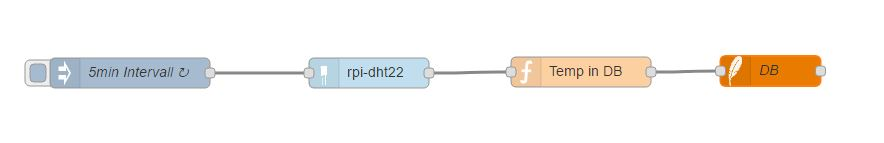
\includegraphics[scale=0.7]{images/tempIntoDB}
	\caption{Temperatur/ Luftfeuchtigkeit in Datenbank}
	\label{flow:tempDB}
\end{figure}
\\\autoref{list:tempIntoDB} zeigt, wie im Funktionsknoten die aktuellen Werte des DHT Sensors aus dem \enquote{msg} Objekt ausgelesen und dem neu erstellen \ac{JSON}-Objekt \enquote{newMsg} im \ac{SQL} Statement übergeben werden. \\Der SQLite Node nimmt anschließend das Event und die neu angelegte Nachricht entgegen und führt den \ac{SQL} Befehl  aus. Dazu muss der \ac{SQL} Befehl immer im zu übergebenen Objekt unter dem Schlüssel \enquote{topic} abgelegt sein. Auffallend hierbei ist, dass anstatt einer ID \enquote{NULL} übergeben wird. Da die Spalte ID Primarschlüssel ist und nicht leer sein darf, wird von SQLite automatisch die neue ID gesetzt.
\begin{lstlisting}[label=list:tempIntoDB, caption={Neuer Eintrag in Tabelle DHT}]
var date = Date.now();
var newMsg = {
"topic": "INSERT INTO DHT VALUES(NULL,"+msg.payload+","+msg.humidity+ ", '"+msg.sensorid+"', "+date+")"
}
return newMsg;
\end{lstlisting}
Der Datenfluss für das Eintragen des Status, ob das Fenster geöffnet oder geschlossen ist (vgl. \autoref{flow:winDB}), hat einen ähnlichen Aufbau wie der Datenfluss in \autoref{flwo:tempDB}. Der Konten \enquote{Pin: 18} sendet immer nur dann ein Event aus, sobald sich eine Zustandsänderung gibt. Damit Rückschlüsse auf die Daten verschiedener Sensoren besser getätigt werden können, speichert der \enquote{Inject}-Node ebefalls im Intervall von 5 Minuten den aktuellen Zustand ab. 
Außerdem stützen mehrere Werte die Genauigkeit von Vorhersagen und Analysen lassen sich leichter generieren, indem in verschiedenen Tabellen nach dem gleichen Zeitstempel gesucht wird.
\begin{figure}[h]
	\centering
	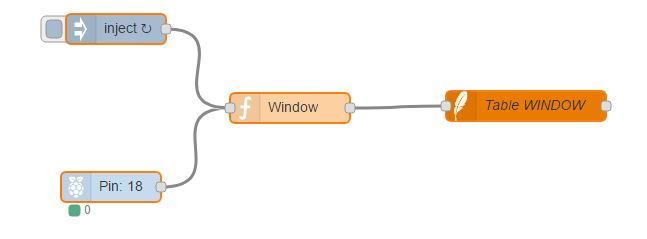
\includegraphics[scale=0.7]{images/windowIntoDB}
	\caption{Fensterstatus in Datenbank}
	\label{flow:winDB}
\end{figure}

Der MQ-135 Sensor gibt ein analoges Signal zurück, das in ein digitales Signal umgewandelt werden muss, damit der Raspberry dieses verarbeiten kann. Es ist also erforderlich, dass ein Analog-Digital-Wandler das Ausgangssignal des Sensors in ein für den Raspberry verständliches digitales Signal umwandelt. Dazu kann der MCP3008 Analog-Digital-Wandler verwendet werden. Da Node-RED hierfür keine Lösung anbietet, werden über Python die Datenbankeinträge für den Sensor erstellt.
\\Eingehende Signale können dann über den \acf{SPI} Bus ausgelesen werden. Der MCP3008 liefert Werte zwischen 0 und 1023 (10Bit) an den Raspberry Pi weiter. Um aus den Werten die Spannung und daraus dann die Gaskonzentration ableiten zu können, ist folgende Formel zu beachten\cite{gas:MQX}:\\
\begin{center} Ausgangsspannung $=  \frac{ADC Wert}{1023} *  $ angelegte Spannung\end{center}

Damit nun die tatsächlichen Gaswerte ermittelt werden können, muss zuerst eine Kalibrierung des Sensors erfolgen. In dieser Phase geht der Sensor davon aus, dass er sich in reiner, guter Luft befindet. Ausgehend von der Kalibrierung gleicht der Sensor dann die ankommenden Daten mit einer speziell für eine Gaswert definierten Geraden ab. Dafür muss aus den Charakteristiken jedes Gases \footnote{Seite 2, https://www.olimex.com/Products/Components/Sensors/SNS-MQ135/resources/SNS-MQ135.pdf} eine entsprechende Geradengleichung ermittelt werden. Die ankommenden Daten eines Gases werden dann mit der entsprechend definierten Geraden des Gases verglichen und die Gaskonzentration ausgegeben.\cite{gas:MQ}. Der Quellcode für die Auswertung der Eingangswerte ist in \autoref{list:MQClass} aufgezeigt.
\\ \autoref{list:MQGas} zeigt den Quellcode auf, der die berechneten Gaswerte in die Datenbank schreibt. Damit Ausreißer nicht ins Gewicht fallen, werden 15 Gaswerte in einem Array gespeichert, sortiert und der Median abgespeichert. Die Generierung eines neuen Datenbankeintrags wird dabei in Zeile 13 dargestellt. In die Datenbank eingefügt wird ein Zeitstempel in Millisekunden, sowie die Werte der verschiedenen Gase.

\begin{lstlisting}[label=list:MQGas, caption={MQ-135 Sensorwerte in DB}]
while True:
	temp = [[], [], []]
	n = 15
	for i in range(n):
		perc = mq.MQPercentage()
		temp[0] += [perc["CO2"]]
		temp[1] += [perc["CO"]]
		temp[2] += [perc["NH4"]]
		time.sleep(2)
	temp[0] = sorted(temp[0])
	temp[1] = sorted(temp[1])
	temp[2] = sorted(temp[2])
	c.execute("INSERT INTO mq135(timestamp, CO2, CO, NH4) VALUES(?, ?, ?, ?)",(int(time.time()*1000), temp[0][int(math.floor((n-1)/2))], temp[1][int(math.floor((n-1)/2))], temp[2][int(math.floor((n-1)/2))]))
conn.commit()
\end{lstlisting}


\subsection{Services Node-RED}
Damit die gespeicherten Daten zu den verschiedenen Sensoren auch für andere Anwendungen bereitgestellt werden können, werden mithilfe des Node-RED-Webservers REST Servies angelegt. Diese können über \ac{HTTP} Anfragen angesprochen werden und liefern als Ergebnis Daten im \ac{JSON}-Format zurück. Dabei wird je nach angesprochenem Pfad ein bestimmtes Ergebnis zurückgeliefert. \\Anfragen müssen an den Raspberry Pi bzw. dessen Webserver-Schnittstelle gesendet werden. Dabei ist darauf zu achten, dass sich der Node-RED-Webserver unter der \ac{IP}-Adresse des Raspberry Pis und dem Port 1880 erreichen lässt. Als Beispiel könnte die Adresse folgendes Format haben: 192.168.0.100:1880. \\Damit nun ein entsprechender Service aufgerufen wird, muss noch eine Pfad an die \ac{URL} angehängt werden. In Node-Red wurden folgende REST \ac{API} Schnittstellen entwickelt:
\begin{itemize}
	\item \textbf{/temp}: Diese Route liefert dem Anwender den aktuell gemessenen Wert vom Temperatur- \& Luftfeuchtigkeitssensor  zurück. 
	\item \textbf{/tempInt}: Um sich den Temperaturverlauf innerhalb eines begrenzten Zeitraums anzeigen zu lassen, kann diese Route angesprochen werden. Dabei müssen ein Startdatum, sowie ein Enddatum jeweils im Format \enquote{dd.mm.yyyy} als Parameter der Anfrage mit übergeben werden.
	\item \textbf{/window}: Gibt den aktuellen Status zurück, ob das Fenster geöffnet oder geschlossen ist.
	\item \textbf{/motion}: Liefert als Ergebnis eine ID und einen Zeitstempel zurück, um dem Anwender mitzuteilen zu welchem Zeitpunkt eine Bewegung erkannt wurde.
	\item \textbf{/picture}: Dieser Service benötigt als Parameter eine ID, die über den Pfad \enquote{/motion} ermittelt werden kann. Durch diese ID kann dann der Pfad zum entsprechenden Bild geladen werden und als Antwort wird das Bild dem Anwender angezeigt.
	\item \textbf{/mqgas}: Die aktuellen Gas-Werte können über den Service herausgefunden werden.
	\item \textbf{/gasInt}: Gleiches Prinzip, wie bei der Route \enquote{/tempInt}. Dem Request werden zwei Parameter (Startdatum, Enddatum) übergeben und die Gaswerte zurückgeliefert, die im angegebenen Zeitraum erfasst wurden.
\end{itemize}

\autoref{flow:TempInt} stellt beispielhaft den Node-RED-Flow zum Abfragen des Temperatur- und Luftfeuchtigkeitsverlaufs dar. Der Service wird angesprochen, wenn folgender Pfad adressiert wird: /tempInt?from=10.05.2017\&to=22.05.2017. Mit dieser Anfrage werden alle gespeicherten Werte als Antwort zurückgeliefert, die im entsprechenden Intervall liegen.
\begin{figure}[h]
	\centering
	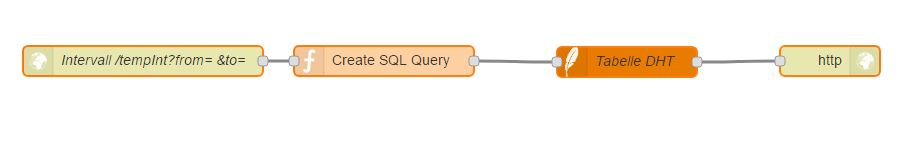
\includegraphics[scale=0.7]{images/tempIntFlow}
	\caption{Beispiel: Temperatur Intervall abfragen}
	\label{flow:TempInt}
\end{figure}
Der erste Node wird dazu benötigt, um eine HTTP Request anzunehmen. Dabei ist die Route zu definieren, unter der der Service erreichbar sein soll. In diese Fall ist dies \enquote{/tempInt}. Die übergebenen Parameter werden erst im Funktionsknoten betrachtet, d. h. die eingehenden Parameter werden über ein JSON-Objekt an den nachfolgenden Knoten übergeben. 
\\\autoref{list:tempInt} ist der Quellcode des Funktionsknotens. In Zeile 3 wird geprüft, ob beide Parameter gesetzt sind. Falls dies nicht der Fall ist, sollen die letzten 20 Einträge aus der Datenbank geladen werden (siehe Zeile 24 \autoref{list:tempInt}). Dieser Schritt ist notwendig, da der nachfolgende Knoten auf die Datenbank zugreift. Liegt keine Abfrage vor, so wird ein Fehler zurückgeworfen und der Flow  unterbrochen. 
\\Falls beide Parameter gesetzt wurden, müssen JavaScript Zeitstempel generiert werden, da nur solche in der Datenbanktabelle DHT gespeichert sind. Hierfür werden in Zeile 10f die beiden Strings in Arrays unterteilt, sodass das Jahr, der Monat und die Tage separiert sind. Anschließend kann mithilfe des Date Objektes ein Zeitstempel generiert werden. Dabei ist darauf zu achten, dass JavaScript in den Monaten bei \enquote{0} zu zählen beginnt und somit der Monat um eins reduziert werden muss. \\Der timestampTo wird außerdem noch mit 23 Stunden, 59 Minuten und 59 Sekunden erzeugt, damit ein einzelner Tag auch respektiert werden kann. \\Sobald beide Zeitstempel vorliegen, wird die \ac{SQL} Abfrage generiert und in der Variable \enquote{selectString} gespeichert. \\Zum Schluss muss die Abfrage in einem JavaScript Objekt als Key-Value übergeben werden. Die Datenbankabfragen müssen dabei immer unter dem Key \enquote{topic} abgelegt sein. Zum Schluss wird das Objekt dann noch zurückgegeben, sodass es vom nächsten Node verwendet werden kann. 
\begin{lstlisting}[label=list:tempInt, caption={Funktion Node-RED tempInt}]
var selectString;

if(msg.req.query.from && msg.req.query.to){
	var fromDate = msg.req.query.from;
	var toDate = msg.req.query.to;
	
	/*convert date into timestamp
	first divide date string into day, month, year 
	then create new Date to get an timestamp*/
	var fDate = fromDate.split("."); 
	var tDate = toDate.split(".");
	
	/*create timestamp; month-1 because Jan = 0, Feb = 1 etc.
	date requires the order: year, month, day, hours, minutes, seconds */
	var timestampFrom = new Date(fDate[2], fDate[1]-1, fDate[0]).getTime();
	//to respect the whole day set hours, minutes, and seconds
	var timestampTo = new Date(tDate[2],tDate[1]-1, tDate[0], 23, 59, 59).getTime();
	
	var select = "Select * FROM DHT WHERE timestamp >= "; 
	var and = " AND timestamp <=";
	selectString =select + timestampFrom + and + timestampTo;
}
else {
	selectString = "Select * FROM DHT ORDER BY ID DESC LIMIT 20";
}

//create Message object for db access
var newMsg = {};
newMsg.topic = String(selectString);
return newMsg;
\end{lstlisting}

Nachdem die Abfrage im entsprechenden Objekt vorliegt, kann der Datenbankknoten die Anfrage verarbeiten und die ermittelten Ergebnisse werden an die \ac{HTTP} Node gesendet. Dabei muss in dem SQLite Node der Pfad zur SQLite Datenbank gesetzt werden.
\\\autoref{list:temp}  zeigt das \ac{JSON}, das vom Webserver als Antwort zurückgeliefert wird. Dieses hat durchgehend die gleiche Struktur und kann somit nach dem Key-Value-Prinzip ausgelesen werden. Enthält eine Antwort mehrere Einträge, wird ein Array mit mehreren Objekten zurückgeliefert.
\begin{lstlisting}[label=list:temp, caption={Beispiel: JSON Response für den Pfad: /temp}]
{
	"temp": "24.60",
	"humidity": "46.60",
	"sensorid": "dht22",
	"date": 1495920298490
}
\end{lstlisting}


\section{Mobile Android Applikation}
Als grafische Benutzerschnittstelle , für das in dieser Arbeit erläuterte System, wird eine ortsunabhängige Lösung entwickelt (F-10.2). Um eine Ortsunabhängigkeit gewährleisten zu können, bietet es sich an, ein mobiles Endgerät zu entwickeln. Es wurde  entschieden als Benutzerschnittstelle eine Android App zu nutzen, da das Android-Betriebssystem den höchsten Endkundenabsatz besitzt \cite{statista:marktanteileandroid} und dadurch eine größere Masse erreicht werden kann.

\subsection{Architektur der mobilen Android Applikation}\chapterauthor{Louisa Pabst}
Auf Grundlage der Anforderungen wird die Architektur der mobilen Android Applikation erstellt.
In der Architektur werden alle wichtigen Entscheidungen, welche für die Entwicklung des Systems relevant und von technischer Natur sind, berücksichtigt. Die Architektur dient als Grundlage für die darauffolgende Umsetzung der Applikation.\\
Um die Anwendung strukturierter entwickeln zu können, wird ein Entwurfsmuster zur Strkturierung der Applikation genutzt. Als Entwurfsmuster bietet sich das \ac{MVC} Entwurfsmuster an. Das \ac{MVC} Designpattern beschreibt eine Architektur zum Anordnen von Objekten. Das \ac{MVC} Entwurfsmuster ermöglicht dabei, einen großen Spielraum für individuelle Anpassungen, weil es nicht starr definiert ist \cite{bucanek:modelviewcontroller}.\\
MVC ermöglicht zwischen der Anzeige der Daten, der Datenverwaltung und der Datenspeicherung eine Unabhängigkeit der Daten zu gewährleisten. So müssen bei Veränderungen des Datenmodells keine Anpassungen an der grafischen Benutzerschnittstelle direkt durchgeführt werden. Es können auch mehrere Views zu einem Model gehören ohne sich gegenseitig zu behindern. Was beachtet werden muss, ist das ein \ac{MVC} Entwurfsmuster bei kleinen Softwareprojekten schnell den Code unnötig aufblasen lässt. Innerhalb dieser Arbeit wird es jedoch als sinnvoll erachtete und genutzt. Zum einen das komplexe Datenmodell und zum Anderen die visuelle Aufbereitung der Daten rechtfertigen die Nutzung eines MVC Musters. Eine Wartung des Quelltextes wird durch ein \ac{MVC} Entwurfsmuster erleichtert, da es hilft den Code übersichtlich aufzuteilen \cite{bucanek:modelviewcontroller}.


\subsection{Rule Engine}\chapterauthor{Louisa Pabst}
Vor Beginn der Entwicklung muss die Struktur von Regeln analysiert werden. Eine Regel besteht aus einem Wenn-Teil und dem Dann-Teil. Der Wenn-Teil wiederum kann aus mehreren einzelnen Wenn-Teile zu einem übergreifenden Wenn-Teil zusammengefasst werden. Das Zusammenfassen mehrerer Wenn-Teilen führt zu mehr Regelmöglichkeiten. Der gleiche Grund kommt bei dem Dann-Teil zum Tragen. Gerade im Hinblick auf die Integration von weiteren Akteuren (F-60.2) ist es sinnvoll, mehrere Akteure innerhalb einer Regel auslösen zu können.\\
Ein einzelner Wenn-Teil der Regel besteht aus einem Datentypen, Vergleichsoperator/en, Vergleichsdaten und einer Konjunktion zu einem anderen Wenn-Teil. Um dem Nutzer eine intuitivere Anwendung bieten zu können, werden Vergleichsoperatoren in Regeln angeboten, die aus zwei Operatoren bestehen. So können Vergleichsoperatoren, wie ``zwischen'' gewährleistet werden. Ein Wert ist dann zwischen zwei Werten, wenn der Datenwert größer als Vergleichswert 1 und kleiner als Vergleichswert 2 ist. Innerhalb der Rule Engine wird dementsprechend zwischen klassischen binären und zusammengesetzten binären Operatoren unterschieden. Binäre Operatoren vergleichen zwei Werte miteinander \cite{unilinz:binaereoperatoren}.\\
Erstellte Regeln werden dem Ersteller direkt zugeordnet. Die Sensordaten sind im Gegensatz nicht Nutzern zugeordnet, sondern einem Raspberry Pi. Das bedeutet mehrere Bewohner eines Hauses können auf die gleichen Sensoren zugreifen, sich aber individuelle Regeln auf ihre Bedürnisse hin definieren.\\
Die Rule Engine wird nach den Anforderungen aus Kapitel \ref{sec:Anforderungen} entwickelt. Demnach muss die Rule Engine dem Nutzer ermöglichen, dynamisch Regeln hinzufügen oder wieder zu löschen zu können. (F-30.1). Grenzwerte oder Wertebereiche kann der Nutzer für die erfassten Datentypen (F-10) selbst bestimmen (F-30.2). Des Weiteren soll die Rule Engine zeitliche Aspekte in den Regeldefinitionen einbinden können. Der Nutzer kann demnach zeitliche Intervalle festlegen, in denen ein Wert oder Wertebereich gehalten werden soll. Die Definition von Datenabhängikeiten kann von der Rule Engine verarbeitet werden, um optimalere Aktionen auslösen zu können (F-30.5).\\
Es werden mögliche Rule Engines recherchiert, die die gestellten Anforderungen erfüllen. Dabei wurden nur Rule Engines betrachtet, die in Android genutzt werden können, sowie welche mit regelmäßigen Releases. Aus der Recherche haben sich folgende Rule Engine Bibliotheken ergeben:
\begin{itemize}                                                                                                               
	\item Easy Rules \cite{github:easyrules}
	\item OpenRules \cite{openrules}
	\item RuleBook \cite{github:rulebook}
\end{itemize}
Diese Rule Engines bieten gute Möglichkeiten Regeln zu erstellen und diese zu überprüfen. Regeln für bestimmte Werte können zur Laufzeit hinzugefügt werden. Dies ist im Hinblick auf die Sensorenerweiterung durchaus sinnvoll. Jede Regel muss jedoch hartcodiert vor der Laufzeit in die Rule Engine hinzugefügt werden. Das ist ein entscheidener Nachteil dieser Rule Engines. Durch die Recherche konnte keine Engine gefunden werden, die eine dynamische Erstellung von neuen Regeln über die Oberfläche ermöglicht. Die Definition neuer Regeln durch den Nutzer ohne den Quellcode zu verändern, ist jedoch eine essentielle Anforderung. Aus diesem Grund wurde sich dafür entschieden, eine Rule Engine selbst zu implementieren.\\
Bei der Implementierung der Rule Engine wurden die Ergebnisse der Recherche miteinbezogen. Vor allem die Struktur der Regeln zu ihren Wenn- und Dann-Teilen der Regel Engine RuleBook wurde bei der Implementierung betrachtet.\\
Für die Strukturierung der Rule Engine wurden mögliche Lösungswege betrachtet. Eine Möglichkeit wäre jede Regel als Java-Klasse zu erstellen. Jede spezifische Regel würde dann von der Klasse Regel erben, sodass die Haupteigenschaften in jeder Klasse erhalten sind. Um dem Nutzer das Hinzufügen einer neuen Regel zur Laufzeit zu ermöglichen,müsste eine neue spezifische Regel-Klasse zur Laufzeit hinzugefügt werden.

Das Hinzufügen von Klassen zur Laufzeit hat vor allem vier Nachteile, die in unserem Kontext relevant sind. Der erste Nachteil ist die Umgebung, in der der Quellcode ausgeführt werden muss. Zur Kompilierung zur Laufzeit muss die Umgebung eine JDK besitzen. Ohne JDK ist das Hinzufügen von Klassen zur Laufzeit nicht möglich. Ein weiterer Nachteil ist die Komplexität. Durch das Kompilieren von Klassen zur Laufzeit entsteht eine erhöhte Komplexität, aus der auch der dritte Nachteil resultiert. Die Geschwindigkeit der Applikation wird beeinträchtigt. Gerade bei einer mobilen Applikation möchte ein Nutzer nicht lange auf das Ergebnis warten. Der letzte entscheidene Nachteil ist die Sicherheit. Wenn dem Nutzer die Möglichkeit gegeben wird zur Laufzeit eine Regel hinzuzufügen, kann dieser versuchen Schadcode einzubauen. Bei erfolgreicher Schadcode-Einbettung ist die gesamte Applikation stark beeinträchtigt.\\
Eine weitere Möglichkeit eine Rule Engine zu implementieren, ist diese mit Hilfe eines JavaScript Interpreters zu realisieren. Die Regel wird dabei in JavaScript Code abgespeichert. Bei Ausführung der Rule Engine wird dann der JavaScript Code interpretiert. Auch bei dieser Möglichkeit der Umsetzung ist die Sicherheit ein entscheidender Nachteil. Es muss verhindert werden, dass der Nutzer bei der Spezifikation der Regel Schadcode einfügen kann, die dann durch den Interpreter ausgeführt wird. Um JavaScript auf einem Android Gerät ausführen zu können, muss ein leichtgewichtiger JavaScript Interpreter gefunden werden, damit die Schnelligkeit der Anwendung nicht darunter leidet. Es wurden Rhino, Nashorn und J2V8 als mögliche  JavaScript Interpreten untersucht.\\
Rhino ist eine JavaScript Engine mit der es möglich ist JavaScript in Java Bytecode zu kompilieren und zur Laufzeit zu interpretieren.\cite{mozilla:rhino}. Rhino lässt sich zudem in Android einbinden. Ein Nachteil von Rhino ist die Komplexität. Innerhalb dieser Arbeit werden nur unkomplizierte if-Abfragen mit einem String Rückgabewert in JavaScript interpretiert werden müssen. Nashorn ist ein Nachfolger des Rhino Interpreters. Nashorn kommt nicht als Interpreter innerhalb dieser Arbeit in Frage, da dieser keine Integration in Android zulässt.\\
Eine weitere Möglichkeit ist die Verwendung der J2V8 JavaScript Engine \cite{github:j2v8}. Diese Engine ist eine leichtgewichtige Form der V8 Engine. V8 ist eine Google Open Source JavaScript Engine \cite{github:v8}. Der entscheidende Vorteil von J2V8 gegenüber der V8 Engine ist die Performanceverbesserung. J2V8 eignet sich dementsprechend gut für die Integration in dieser Arbeit.\\
Um die J2V8 Engine nutzen zu können, muss eine Laufzeitumgebung erstellt werden. Zu dieser Umgebung kann anschließend JavaScript Code hinzugefügt werden, der ausgeführt wird. Dabei muss angegeben werden um welchen Rückgabewert es sich handelt. Der Rückgabewert wird dann an den Java Code übergeben. Durch die Interpretation von JavaScript kann die Rule Engine auf eine Methode reduziert werden. Im Folgenden Code ist diese aufgezeigt.
\begin{lstlisting}[language=java]
	public void run(HashMap<String, String> values){
		PushMessage push = new PushMessage();
    	V8 runtime = V8.createV8Runtime();
        List<String> rules = db.getRuleStrings(db.getloggedInUser());
        Iterator it = values.entrySet().iterator();
        while (it.hasNext()) {
            Map.Entry entry = (Map.Entry) it.next();
            variables += "var " + entry.getKey().toString() + " = " + entry.getValue() + ";";
        }
        for (int r = 0; r < rules.size(); r++) {
            String rule = rules.get(r);
            String notificationText = runtime.executeStringScript(variables + rule);
            runtime.release();
            if(!notificationText.isEmpty()) {
                push.sendNotification(notificationText);
        }
    }
\end{lstlisting}
Die Überprüfung einer Regel wird in drei Schritten durchgeführt.
\begin{enumerate}
\item Im ersten Schritt werden die Variablen der JavaScript Umgebung hinzugefügt. Die Variablen sind die Datentypen, die von den Sensoren übergeben werden. Auf die genaue Kommunikation der Daten von Node-RED zur Regel Engine wird später eingegangen. Die Regel Engine kann dabei unterschiedliche Datentypen übergeben bekommen, die nicht fest definiert sein müssen. 
\item Im zweiten Schritt wird die Regel in JavaScript Format ausgeführt. Die Regel ist eine if-Abfrage, die bei Erfüllung der Kondition einen Text ausgibt. Der Text beinhaltet den Handlungsvorschlag an den Nutzer.
\item Im dritten Schritt wird eben dieser Handlungsvorschlag an die Java Umgebung zurückgegeben, um dem Nutzer über eine Benachrichtigung den Handlungsvorschlag zu eröffnen.
\end{enumerate}

\subparagraph{Kommunikation der Sensordaten}
Im Folgenden wird näher auf die Kommunikation der Sensordaten von Node-RED an die App zur Regelkontrolle eingegangen.\\
Die Daten müssen gebündelt an die App kommuniziert werden.\\
Entweder können die Daten nach einem bestimmten Zeitintervall von der App durch einen HTTP Request eingefordert werden oder durch Node-RED die Daten in regelmäßigen Zeiteinheiten an die App gesendet werden. Es wurde sich innerhalb dieser Arbeit dafür entschieden die Nachrichten von Node-RED schicken zu lassen, damit im Hintergrund der App so wenig wie möglich von der App ausgeführt werden muss. Gerade bei mobilen Applikationen muss darauf geachtet werden, die Batterie und die Netzanbindung so gering wie möglich zu belasten. \\
Die Daten werden im JSON-Format mit Hilfe von \ac{FCM} an die App gesendet \cite{firebase:gcm}. Der zeitliche Rythmus der Datenversendung kann über das Node-RED Interface eingestellt werden. \ac{FCM} bietet drei Möglichkeiten an, das Ziel der Nachricht zu definieren.
\begin{itemize}
	\item Nutzersegment: Nachricht wird an alle geräte eines bestimmten Nutzersegmentes versendet
	\item Thema: Nachricht wird an alle Geräte gesendet, die sich zu einem Thema aboniert haben
	\item Einzelnes mobiles Gerät: Nachricht wird an ein einzelnes Gerät gesendet
\end{itemize}
Für Testzwecke wurde sich entschieden, die Nachrichten an einzelne Geräte zu versenden. Wenn ein Sensorsystem jedoch mehrere Nutzer besitzt, bietet es sich an für jedes Sensorsystem ein Thema zu erstellen, zu dem sich die Nutzer registrieren können.\\
Die Abbildung \ref{fig:sequenzdiagramm} zeigt in Form eines Sequenzdiagrammes den Verlauf von der Übermittlung
der Daten von Node-RED an die App bis zur Auslösung der Aktion an.
\begin{figure}
	\centering
	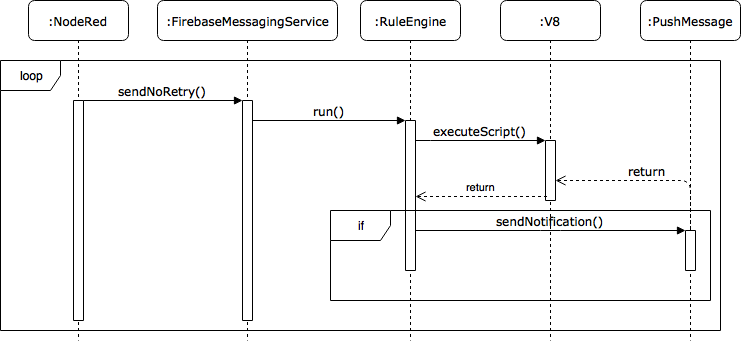
\includegraphics[width=1\textwidth]{images/Sequenzdiagramm.png}
	\caption{Sequenzdiagramm zur Regelkontrolle}
	\label{fig:sequenzdiagramm}
\end{figure}

Bei der Häufigkeit der Benachrichtigungen an den Nutzer muss darauf geachtet werden, dass nicht zu viele Nachrichten an den Benutzer geschickt werden. Bei einer zu großen Häufigkeit an Benachrichtigungen kann der Nutzer diese als eine Belästigung ansehen \cite{gadgets:amountnotifications}. Eine geeignete Anzahl an Benachrichtigungen kann als feste Zahl nicht genannt werden und sollte an den Use Case so gut wie möglich angepasst werden.

\subsection{Daten Anzeige}\chapterauthor{Dominic Steinhauser}
\autoref{label:main} zeigt die Startseite der Anwendung. Sie bietet schnellen Zugriff auf alle ausführbaren Aktionen in der App.
\\Beim Aufrufen der \enquote{AirQuality}-View wird eine \ac{HTTP} Anfrage an den Webserver gesendet. Die zurückgelieferten Ergebnisse, welche den aktuell gemessenen Sensorwerten entsprechen, werden in \autoref{label:airquality} neben ihrer Beschreibung dynamisch gesetzt und liefern so dem Anwender erste Informationen zu seiner Umgebung. Da allerdings nur die aktuellen Sensorwerte in dieser Ansicht angezeigt werden, kann der Anwender über den Pfeil zur nächsten Seite navigieren, die es dann ermöglicht den Verlauf der Daten anzuzeigen. Aus einem Diagramm lassen sich die Werte schnell und einfach ablesen. Außerdem zeigt ein Verlauf, wie sich die Daten im Verhältnis zur Zeit entwickelt haben.

\begin{minipage}[c]{0.5\textwidth}
	\centering
	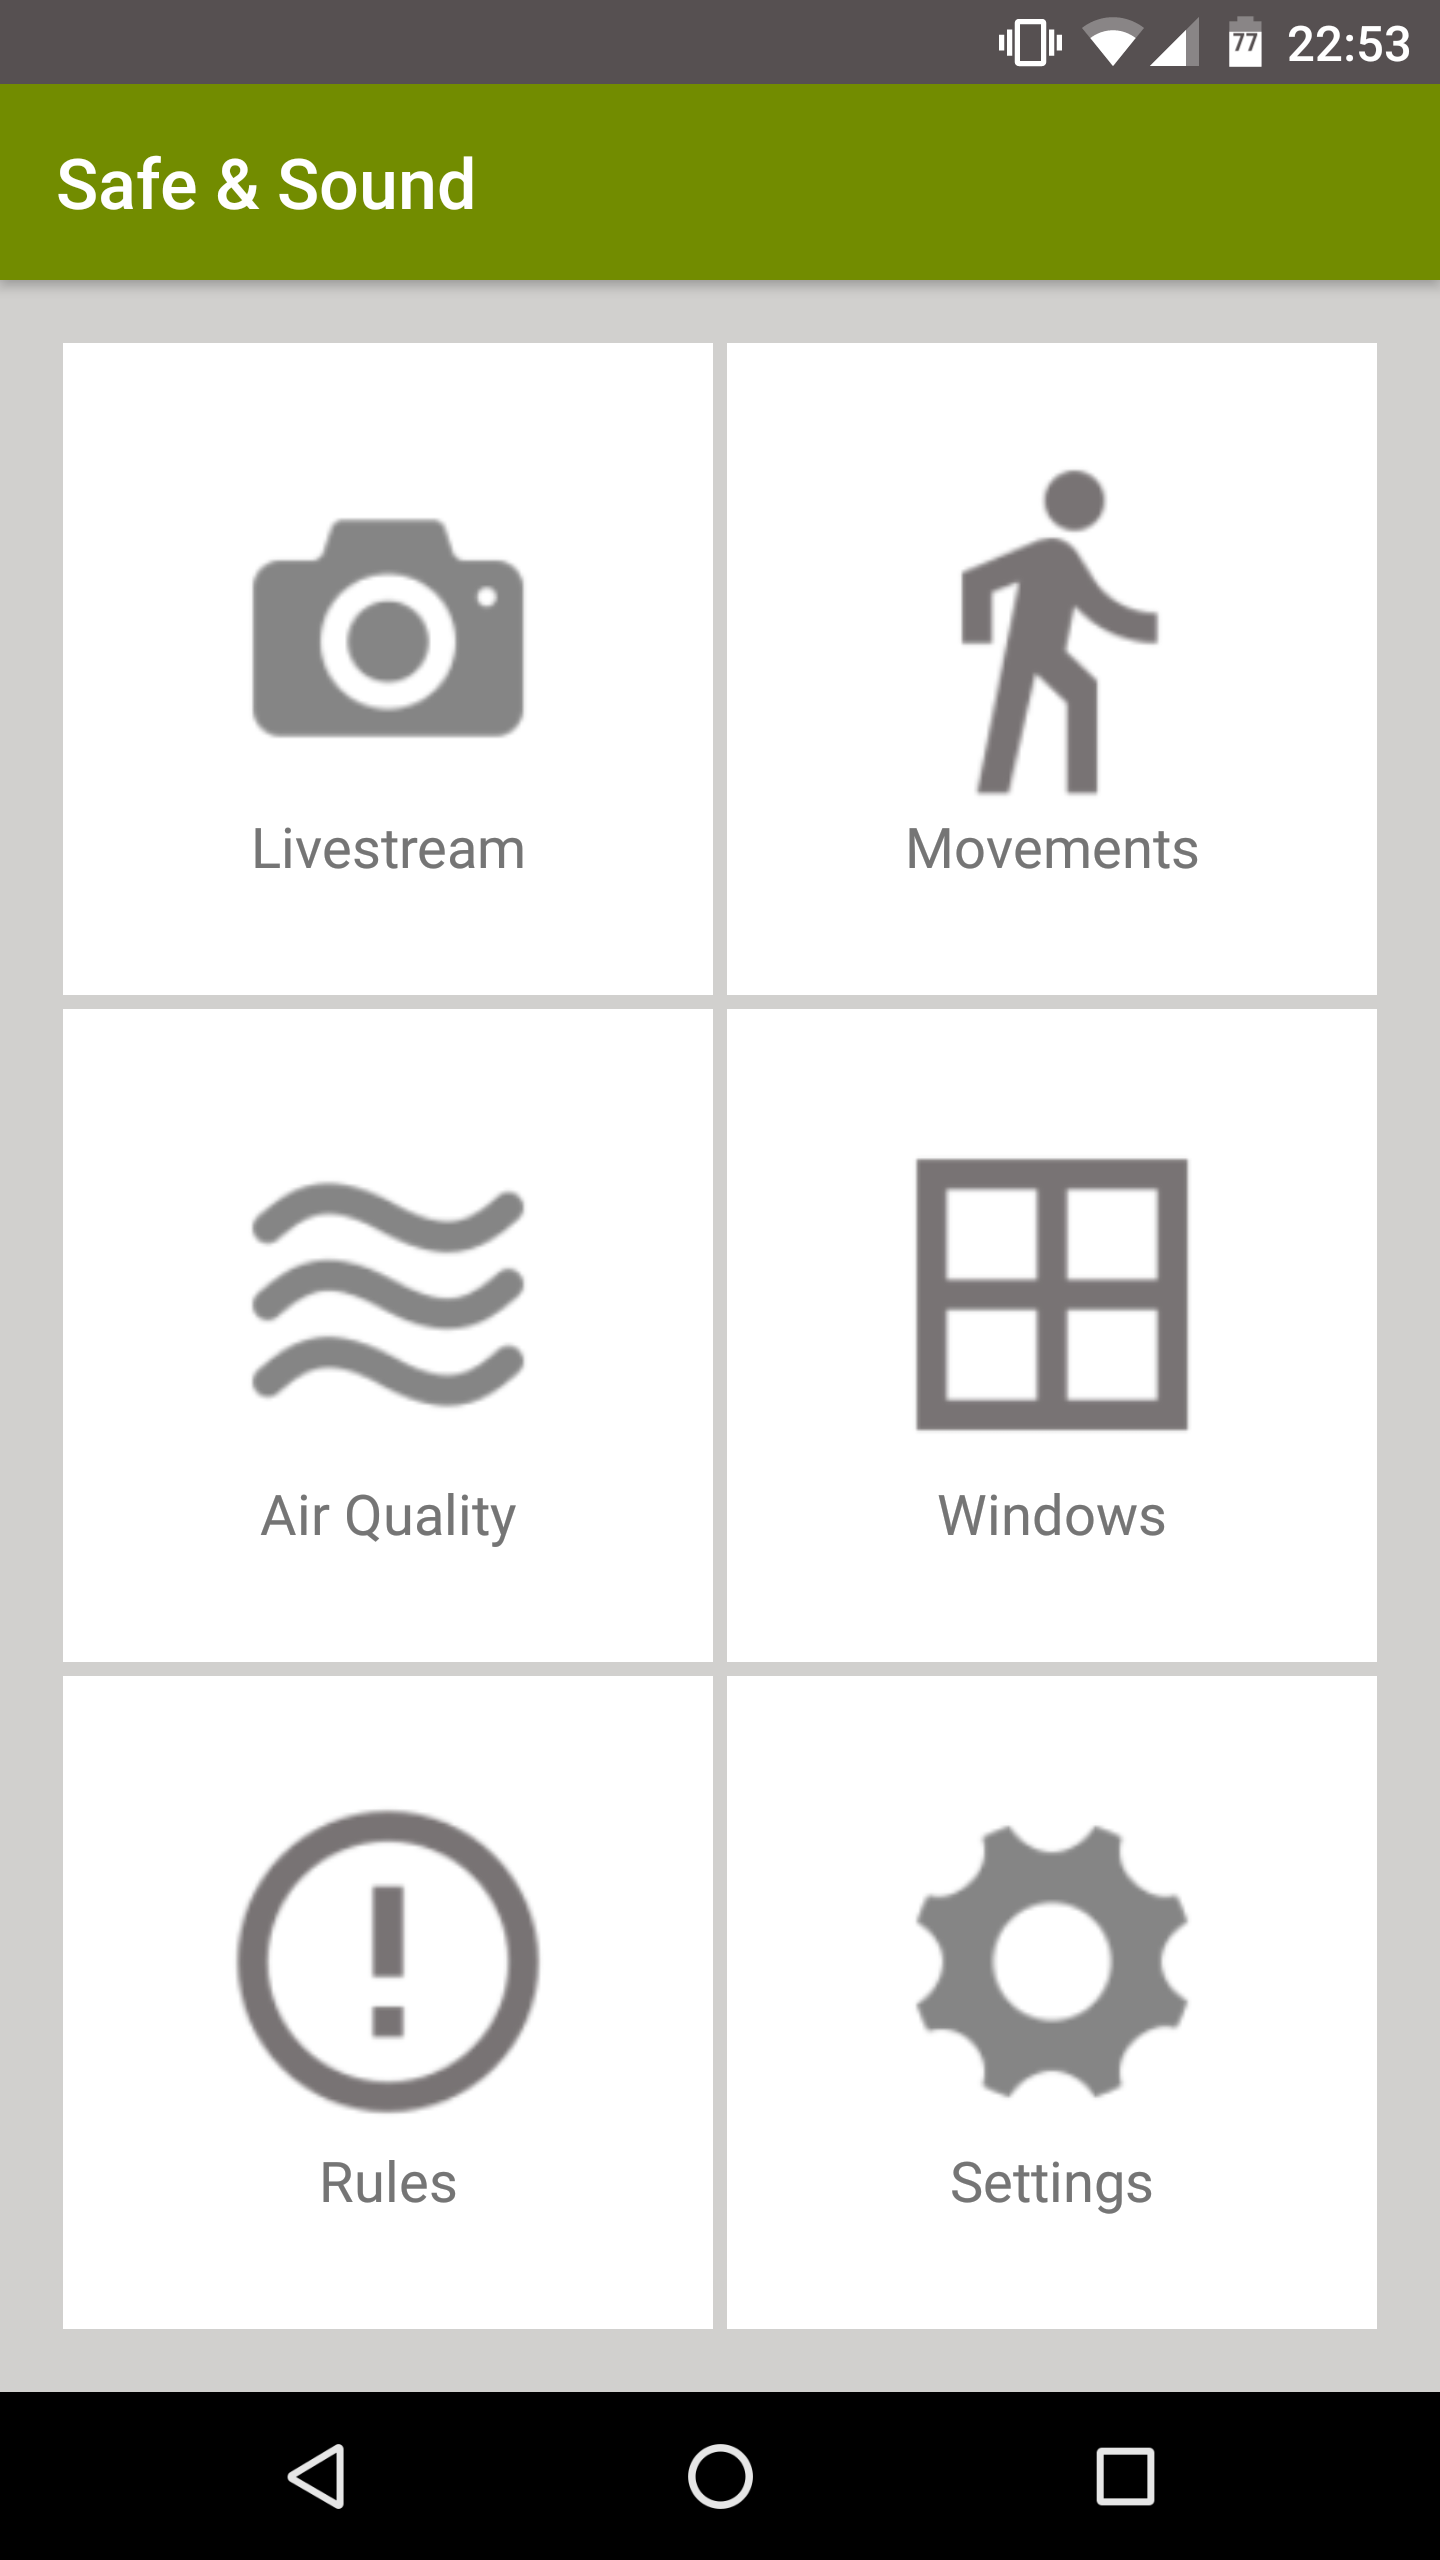
\includegraphics[scale=0.1]{images/appMain}
	\captionof{figure}{Startseite der App}
	\label{label:main}	
\end{minipage}
\begin{minipage}[c]{0.5\textwidth}
	\centering
	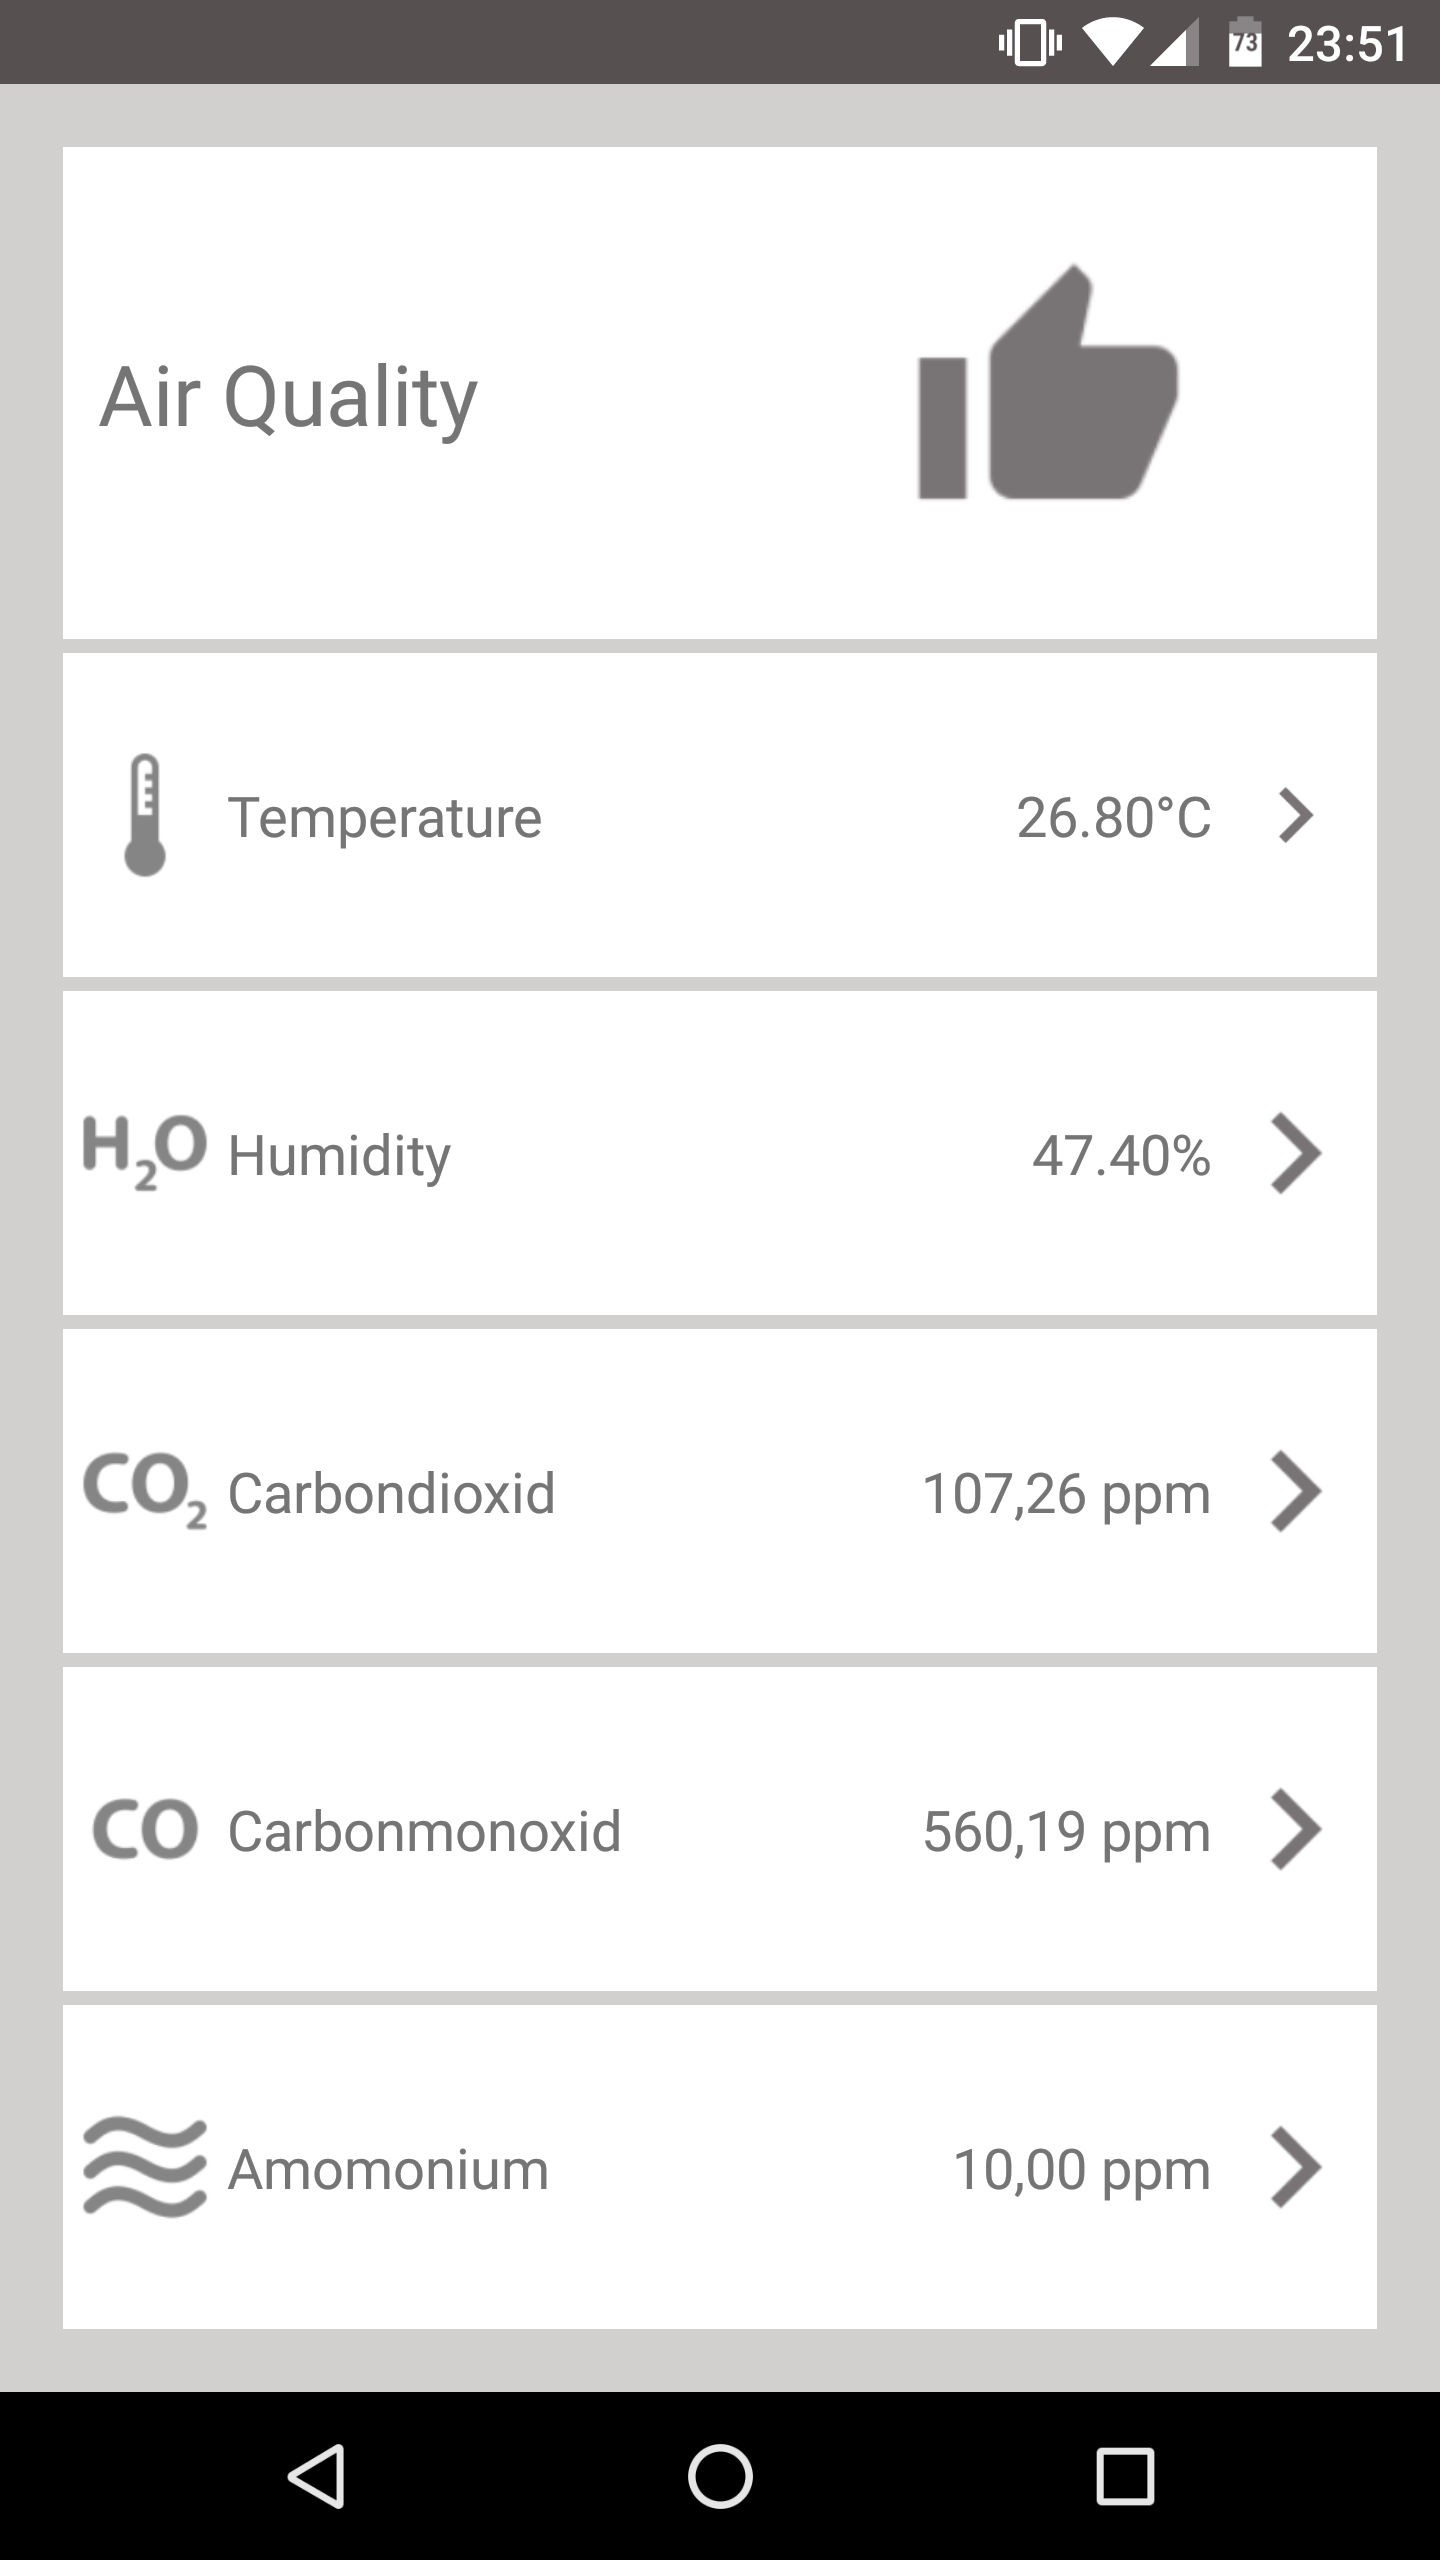
\includegraphics[scale=0.1]{images/airQuality}
	\captionof{figure}{AirQuality}
	\label{label:airquality}
\end{minipage}

Bevor dem Benutzer Daten angezeigt werden, muss dieser zuerst ein Intervall angeben. Dazu wird eine Eingabe über ein Start, sowie ein Enddatum notwendig. Wird nach erfolgreicher Auswahl des Intervalls der \enquote{Show Data} Button geklickt, siehe \autoref{label:tempVerlauf}, wird an den Webserver eine \ac{HTTP} Anfrage geschickt, die entweder für den angegebenen Zeitraum alle Temperatur und Luftfeuchtigkeitswerte oder MQ-135 Daten in einem \ac{JSON}-Array zurückliefert. 

\begin{figure}[h]
	\centering
	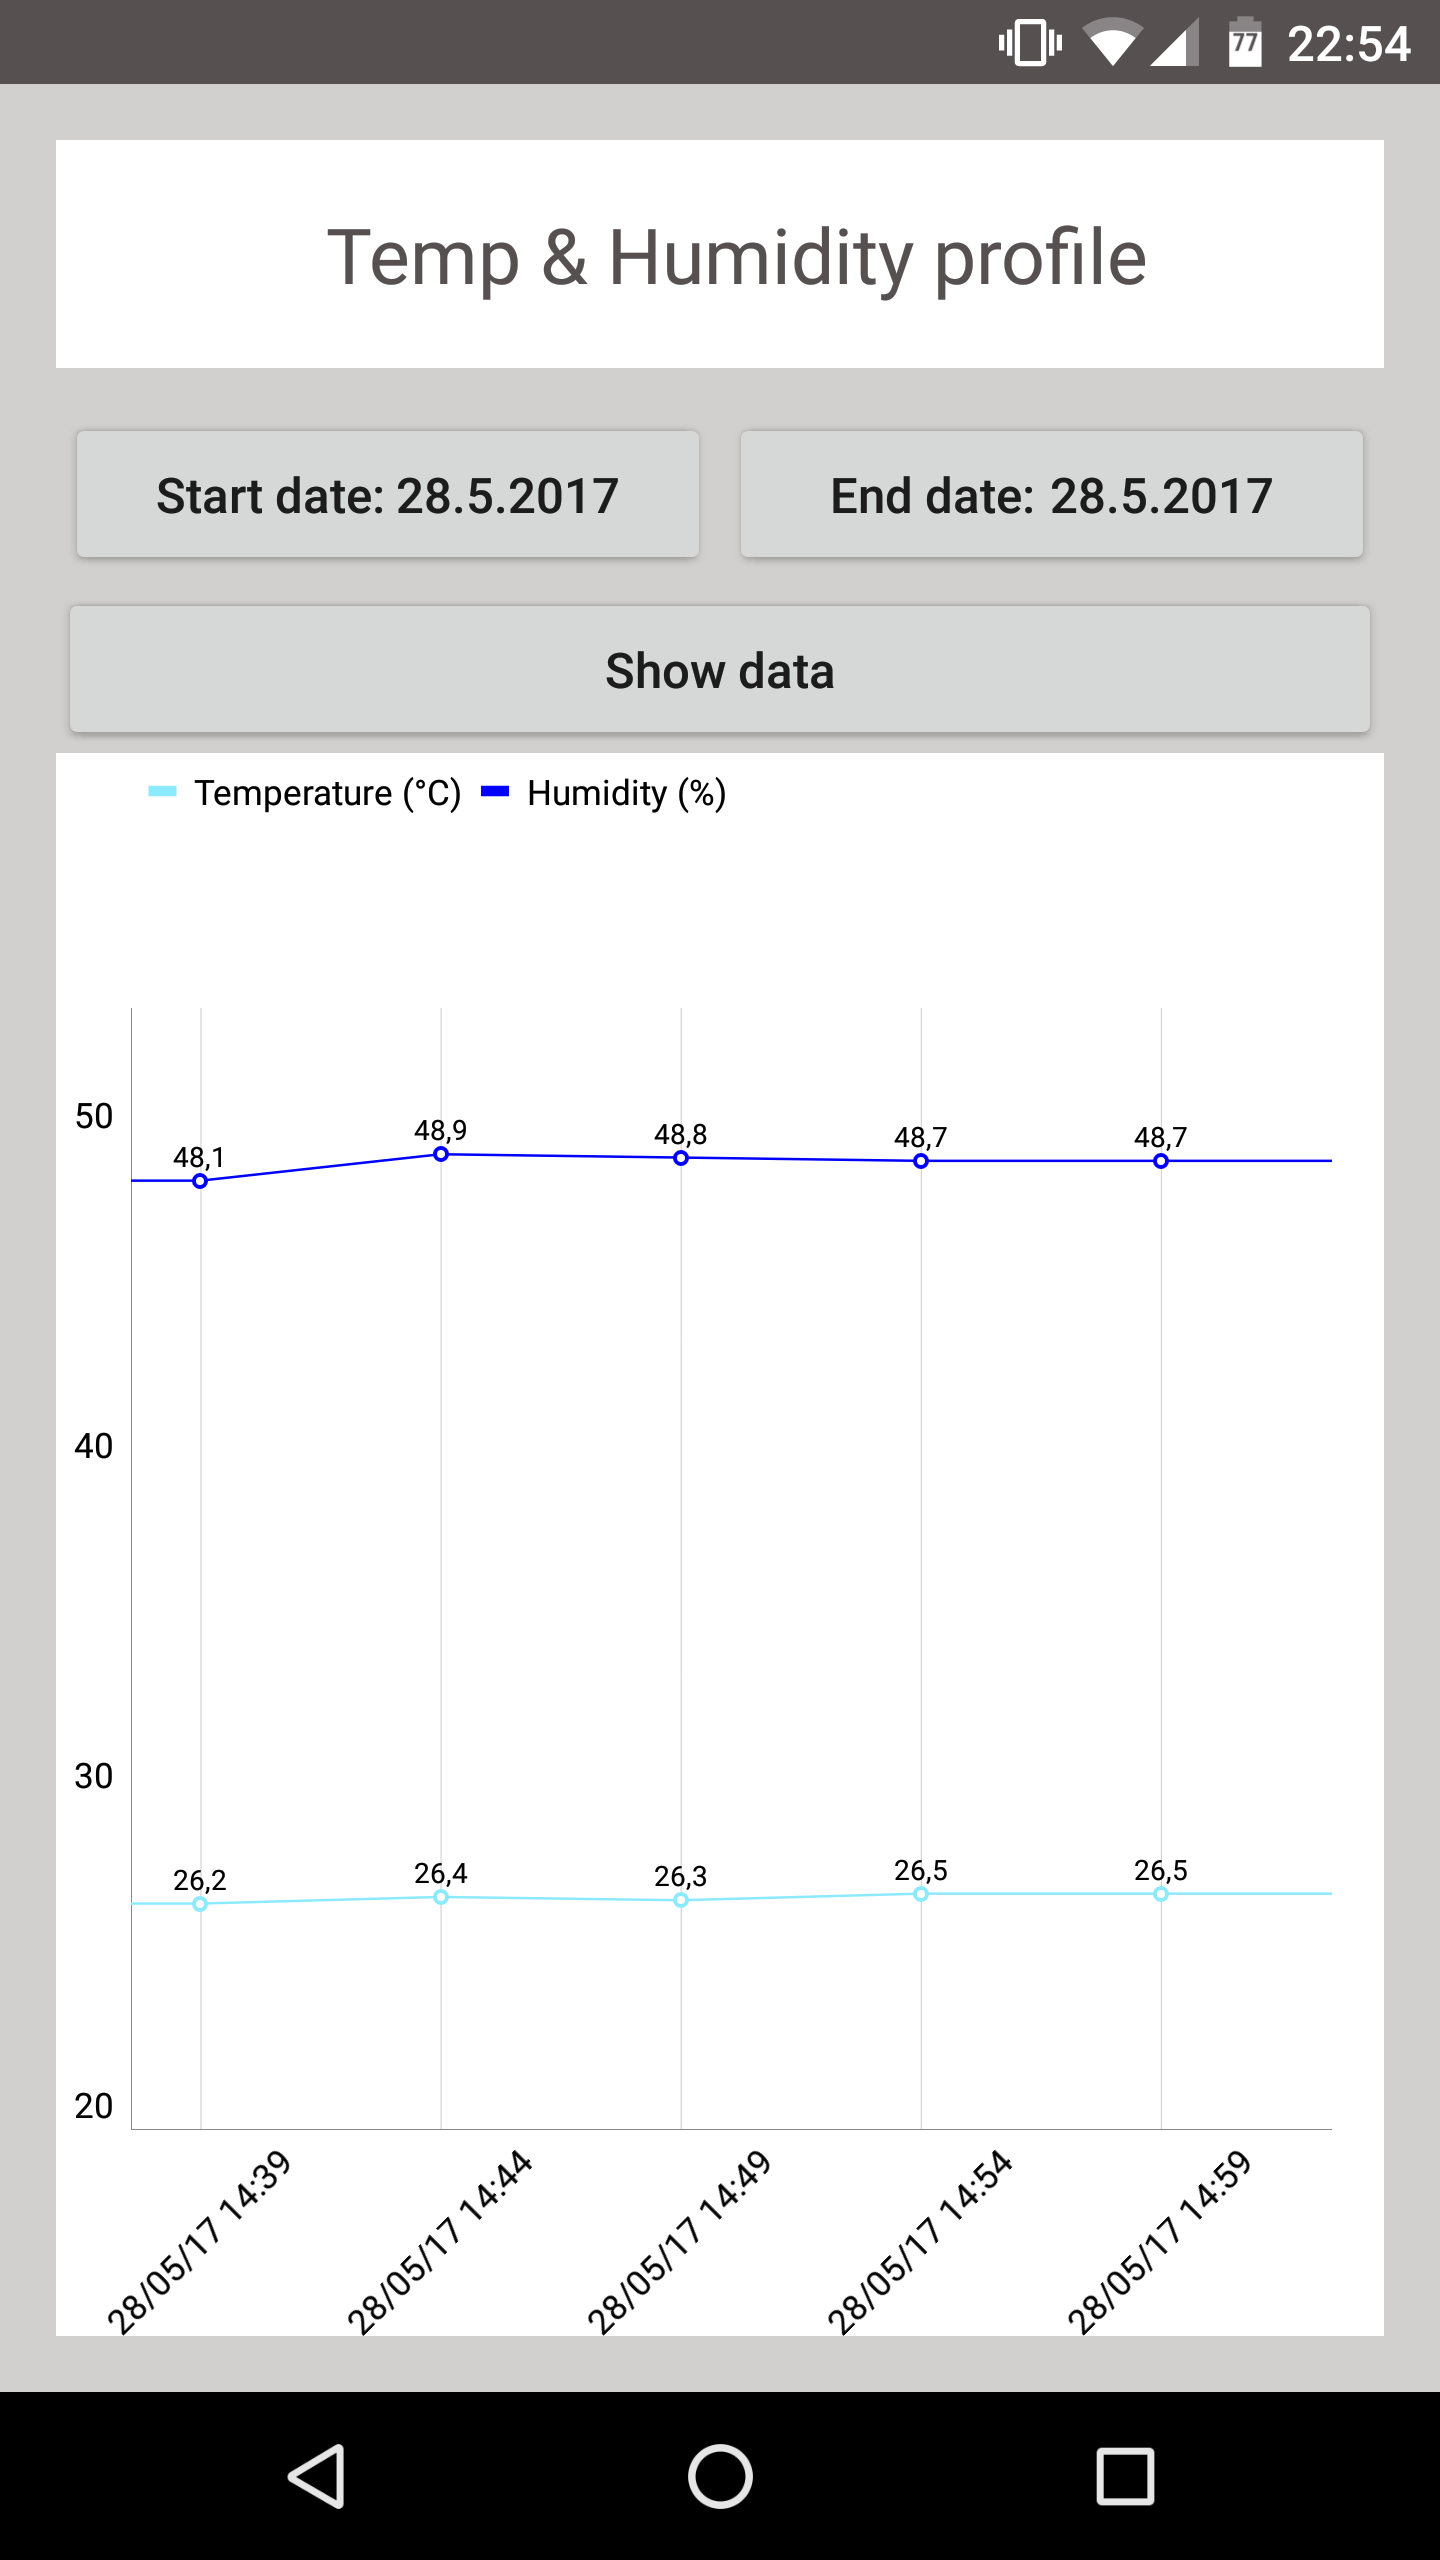
\includegraphics[scale=0.1]{images/appVerlauf}
	\caption{Diagramm Temperaturverlauf}
	\label{label:temVerlauf}
\end{figure}

\autoref{list:Array} zeigt als Beispiel das \ac{JSON}-Array auf, das vom Webserver als Response gesendet wird. 
\begin{lstlisting}[label=list:Array, caption={Beispiel: JSON Array}]
[
	{
		"id": 1184,
		"temperature": 25.8,
		"humidity": 47.9,
		"sensorid": "dht22",
		"timestamp": 1495971295531
	},
	{
		"id": 1185,
		"temperature": 25.8,
		"humidity": 47.9,
		"sensorid": "dht22",
		"timestamp": 1495971595619
	},
	{
		"id": 1186,
		"temperature": 25.9,
		"humidity": 47.8,
		"sensorid": "dht22",
		"timestamp": 1495971895672
	}
]
\end{lstlisting}

Damit nun die Daten in einem Liniendiagramm grafisch dargestellt werden können, ist es notwendig eine Bibliothek zum Visualisieren zu verwenden. Dabei viel die Auswahl auf \enquote{MPAndroidChart}\footcite{https://github.com/PhilJay/MPAndroidChart}. Allerdings gibt es viele verschiedene Bibliotheken, die als Open-Source-Software sich für diesen Zweck eignen.\\
Sobald die Webserver Response als String vorliegt, kann die in \autoref{label:getTem} aufgezeigte Funktion mit der Auswertung des Arrays beginnen. Dabei wird innerhalb der For-Schleife aus jedem \ac{JSON} Objekt der Temperatur- und Luftfeuchtigkeitswert ausgelesen. Die jeweiligen Werte müssen dann der entsprechenden ArrayListe als Entry übergeben werden (vgl. \autoref{label:getTem} Zeile 8ff). Ein Entry entspricht dabei einem Tupel aus zwei Werten für die x und y Koordinate.\\Nachdem alle Werte in der ArrayList \enquote{tempList} bzw. \enquote{humidityList} gespeichert sind, muss eine neue LineDataSet erzeugt werden, die passend zu den Werten noch eine Beschreibung hinzufügt. \\
Damit nun beide LineDataSets in einem Diagramm angezeigt werden können, wird in Zeile 22 eine neue ArrayListe definiert und bei LineDataSets hinzugefügt. Abschließend ein neues LineData Object erstellt und zurückgegeben werden. 

\begin{lstlisting}[label=label:getTem][h]
public LineData getTemHumDataForDiagramm(String s){

	List<Entry> tempList = new ArrayList<Entry>();
	List<Entry> humidityList = new ArrayList<Entry>();
	
	try{
		JSONArray jsonMainNode = new JSONArray(s);
		for(int i = 0; i < jsonMainNode.length(); i++){
			JSONObject jsonChildNode = jsonMainNode.getJSONObject(i);
			Float temperature = BigDecimal.valueOf(jsonChildNode.getDouble("temperature")).floatValue();
			tempList.add(new Entry((float)i, temperature));
			Float humidity = BigDecimal.valueOf(jsonChildNode.getDouble("humidity")).floatValue();
			humidityList.add(new Entry((float)i, humidity));
		}
	} catch (JSONException e){
		Toast.makeText(getApplicationContext(), "Error" + e.toString(), Toast.LENGTH_SHORT).show();
	}
	
	LineDataSet dataSetHum = new LineDataSet(humidityList,"Humidity (%)");	
	LineDataSet dataSetTemp = new LineDataSet(tempList,"Temperature (C)");
		
	List<ILineDataSet> dataSets = new ArrayList<ILineDataSet>();
	dataSets.add(dataSetTemp);
	dataSets.add(dataSetHum);
	
	LineData data = new LineData(dataSets);
	
	return data;
}
\end{lstlisting}

Damit nun die Daten im Diagramm angezeigt werden, müssen dem LineChart Objekt über die Methode \enquote{setData} die Daten übergeben werden. 
\begin{lstlisting}[label=list:showData]
LineChart chart = (LineChart) findViewById(R.id.chart);
LineData data = getTemHumDataForDiagramm(String s)
chart.setData(data)
\end{lstlisting}

